%\documentclass[a4paper,12pt,man]{apa}
\documentclass[a4paper,11pt]{article}

\usepackage{subfigure}

%\usepackage[english]{babel}
\usepackage{setspace}
\doublespacing
%\singlespacing
%\onehalfspacing

\usepackage{amsmath}
\usepackage{amssymb}
\usepackage{amsbsy}

%\usepackage{utopia}
\usepackage{xltxtra}
\usepackage{fontspec}


%\setsansfont[Mapping=tex-text]{Myriad Pro}
\setmainfont[Mapping=tex-text]{Minion Pro}
%\usepackage[math-style=TeX]{unicode-math}
%\setmathfont[]{Cambria Math}

\usepackage{color}
\definecolor{darkblue}{rgb}{0, 0, 0.4}

%\usepackage{times}
\usepackage[colorlinks=true,linkcolor=darkblue,urlcolor=darkblue,citecolor=darkblue]{hyperref}



%\usepackage[math-style=TeX]{unicode-math}
%\setmathfont[]{Asana Math}


\title{Standard errors and confidence intervals for standardized parameters
 in structural equation models}
\author{Daniel Oberski\\Universitat Pompeu Fabra, Spain}
%\date{}
\usepackage[margin=2.8cm]{geometry}

\usepackage{tabularx}

\bibliographystyle{apalike}
\usepackage{natbib}
\usepackage{siunitx} %for \num
\usepackage{rotating}

\newcommand{\n}{\eta}
\renewcommand{\l}{\lambda}
\renewcommand{\b}{\beta}
\newcommand{\p}{\phi}

\renewcommand{\d}{\,\mathrm{d}\,}

\newcommand{\definedas}{\equiv}
\newcommand{\kronprod}{\otimes}
\newcommand{\hadaprod}{\circ}

\newcommand{\diag}{\mathrm{diag}}
\renewcommand{\vec}{\mathrm{vec}\,}
\newcommand{\vech}{\mathrm{vech}\,}

\newcommand{\Lambdastan}{\tilde{\Lambda}}
\newcommand{\Bstan}{\tilde{B}}
\newcommand{\Phistan}{\tilde{\Phi}}
\newcommand{\Psistan}{\tilde{\Psi}}
\newcommand{\thetastan}{\tilde{\theta}}

\newcommand{\0}{\boldsymbol{0}}

\newcommand{\var}{\mathrm{var}}
\newcommand{\arctanh}{\mathrm{arctanh}}

\newcommand{\R}{\texttt{R} 2.13.0 64-bit \citep{R}\;}
\newcommand{\lavaan}{\texttt{lavaan} 0.4.8 \citep{lavaan}\;}

\begin{document}
\maketitle
\newpage

%\marginpar{Beter motiveren; quote Bentler}
\begin{abstract}\noindent
In structural equation models (SEM), the standard errors not only of parameters of the model, but
also of standardized parameters may be of interest to the researcher. 
Examples are the comparison of reliability coefficients across different groups, and meta-analysis of 
standardized quantities.
The literature does not, however, provide explicit analytical standard errors 
for standardized parameters. %Due to this lack of availability of analytical derivatives in the literature, standard SEM software that wishes to provide SEM users with standard errors of the standardized parameters requires the use of numerical derivatives or approximate methods.

We provide the analytical asymptotic variance matrix of standardized parameters in SEM, 
expressed only in terms of the model parameters. The expression is straightforward to 
implement in standard SEM software. 
The asymptotic variance matrix of Fisher $z$-transformed standardized parameters is also provided, 
allowing for the construction of confidence intervals.
We demonstrate the use of the derived expression on an example analysis of the
reliability of self-rated health in groups with different levels of education.
\end{abstract}

\section{Introduction\label{sec:introduction}}\noindent
Linear structural equation models (SEM) with latent variables
have become a popular tool in the behavioral sciences. Such models encompass as special cases a diverse range of common models of interest such as factor
analysis, multivariate regression, errors-in-variables models, growth, and
multilevel and multigroup models \citep{bollen1989structural}. Extensions are available for categorical, count,
and censored dependent variables as well as complex sampling 
 \citep{muthen1995complex,muthen2002beyond}.

Researchers' interest often focuses on the so-called 
`standardized' parameters of the model \citep{bollen1989structural}. Typical applications include examination of factor loadings and correlations in factor analysis, as well as the evaluation of the relative size of regression coefficients, possibly of latent variables.

Although the general principle applied here to derive standard errors and confidence intervals for standardized parameters is well known  \citep[e.g.][]{oehlert1992note}, to our knowledge the literature does not provide any explicit expression for the asymptotic standard errors of standardized coefficients in SEM. As a consequence, standard errors and confidence intervals for these coefficients are usually not provided by the standard software\footnote{At the time of writing, the exception is Mplus version 5.2 and above \citep{muthen1998mplus}.}.  We remedy this situation by deriving an explicit expression, in terms of the unstandardized parameter estimates, for the asymptotic variance-covariance matrix of the standardized coefficients. The solution requires only the parameter estimates of the model and can be readily implemented in SEM software.

Section \ref{sec:example}  provides a motivating example, using a SEM model with latent
variables where standardized parameters and their standard errors and confidence
intervals are of interest to the researcher.
Section \ref{sec:analytics} derives the explicit expression for the asymptotic variance-covariance matrix of the standardized estimates. Section \ref{sec:application} applies this expression to the example. A Monte Carlo study summarized in section \ref{sec:montecarlo}
then evaluates the performance of the analytical standard errors and confidence intervals given here 
by simulation.
Finally, the last section concludes, discusses the scope and limitations of this proposal, and suggests future research.


\section{Example SEM with interest in standardized parameters\label{sec:example}}


Several researchers in public health have studied differences  in self-rated health across societal groups.   For example,  \cite{von2006education} 
compare people with different incomes, age groups, and level of education.
It is well-known, however, that in order to be able to compare correlations across groups it is necessary for the reliability of 
the measures to be the same \citep[e.g.][]{steenkamp1998assessing,saris_design_2007}. 
For example, for comparisons of correlations between self-rated health and other measures
across groups with different levels of educations to be meaningful, the reliability
of self-rated health should be equal for people with different educational attainments.
Therefore not only between-group comparison of the levels of self-rated health are of interest, 
but also the evaluation of differences between the groups in reliability \citep{lundberg1996assessing}. 

Different types of designs exist to estimate the reliability of survey measures. One such design is the repeated measures design, wherein the
same question is asked at least three times with a certain suitably long interval: once a year, for, instance. 
One can then apply the so-called `quasi-simplex' model in different groups to the estimate
reliability, and compare reliabilities across groups \citep{heise1970validity,wiley35wiley}. For an overview of other designs for the estimation of reliability of single questions we refer to \cite{alwin_margins_2007}. 

The quasi-simplex model can be formulated and estimated as a multiple-group structural equation model for groups with different  levels of highest completed education. This model is shown for four repetitions in figure 
\ref{fig:model}. Following \cite{wiley35wiley}, the unstandardized error variances are restricted to be equal across the four repetitions. The reliability coefficients of interest are then the standardized loadings. 
\if 1=2
\begin{eqnarray*}\begin{split}
\textbf{y} =  \textbf{I} {\eta} + \epsilon,& &
{\eta} = \begin{pmatrix}
	0 & 0 & 0 & 0\\
	\beta_{21} & 0 & 0 & 0\\
	0 & \beta_{32} & 0 & 0\\
	0 & 0 & \beta_{43} & 0\\	
\end{pmatrix} {\eta} + \zeta
\end{split}
\end{eqnarray*}
\fi


\begin{figure}[bt]\begin{center}
\caption{Quasi-simplex model for four repeated measures of self-rated health in the LISS panel 2007--2010. Parameter names for the 
	so-called `stability coefficients' are shown as $\beta_{ji}$ in the picture. The variances of the disturbance terms $\zeta_i$ are denoted
	$\phi_{ii}$, while the variances of the measurement error variables $\epsilon_i$ will be denoted $\psi$.}
\label{fig:model}
\includegraphics[width=.9\textwidth]{self-rated-health-quasi-simplex}
\end{center}
\end{figure}

We estimate this model using the LISS panel study, a probability sample 
of 8735 Dutch citizens, who regularly answer questionnaires over the web. 
For more information about the LISS we refer to \cite{scherpenzeel2011data}.
The  panel contains a study that included the commonly used self-rated health question\footnote{The original question was asked in Dutch. See \url{http://www.lissdata.nl/dataarchive/question_constructs/view/600}}. The question was asked as follows:
\begin{quote}
	How would you describe your health, generally speaking?
	
	\begin{enumerate}  \setlength{\itemsep}{0pt}  \setlength{\parskip}{0pt}
  \setlength{\parsep}{0pt}
		\item Poor
		\item Moderate
		\item Good
		\item Very good
		\item Excellent
	\end{enumerate}
\end{quote}


\begin{table}[bt]\begin{small}
\begin{center}
\begin{tabular}{llrrrrrrrrr}  \hline  \hline
&&&  \multicolumn{8}{c}{\emph{Year}}\\\cline{4-11}
&&& \multicolumn{2}{c}{2007} & \multicolumn{2}{c}{2009} & \multicolumn{2}{c}{2009} & \multicolumn{2}{c}{2010} \\
&&$n$&Mean&sd&Mean&sd&Mean&sd&Mean&sd\\
%&	&	Primary		&VMBO		&		MBO	&HAVO/VWO&	HBO	&	WO	\\	
  \hline
  \multicolumn{2}{l}{Education level}\\
 
& Primary	  & 279 & 2.83 & (0.69) & 2.91 & (0.73) & 2.84 & (0.74) & 2.82 & (0.72) \\ 
& Lower secondary  & 940 & 2.98 & (0.73) & 3.08 & (0.73) & 3.01 & (0.71) & 2.97 & (0.73) \\ 
& Middle secondary & 782 & 3.21 & (0.80) & 3.24 & (0.76) & 3.27 & (0.81) & 3.20 & (0.75) \\ 
& Upper secondary  & 369 & 3.17 & (0.75) & 3.18 & (0.74) & 3.16 & (0.72) & 3.10 & (0.72) \\ 
& Lower tertiary	  & 799 & 3.28 & (0.73) & 3.28 & (0.76) & 3.22 & (0.72) & 3.22 & (0.74) \\ 
& Upper tertiary	  & 256 & 3.33 & (0.86) & 3.35 & (0.86) & 3.32 & (0.82) & 3.29 & (0.83) \\ 
   \hline
   \hline
\end{tabular}
\caption{Means and standard deviations (in brackets) of the self-rated health question across the four repetitions (2007--2010), in 
groups with different levels of education.}\label{tab:descriptives}
\end{center}\end{small}
\end{table}

This question was asked of 3425 LISS respondents in the years 2007, 2008, 2009, and 2010. 
Table \ref{tab:descriptives} shows the mean and standard deviation of self-rated health in
groups with six different levels of education.
We estimate the quasi-simplex model shown in figure \ref{fig:model} as a multiple group SEM
to yield four standardized loadings for each of the six educational groups, which can be interpreted as the reliability coefficients for each group\footnote{For the estimation we used \R and \lavaan}. The unstandardized parameter estimates and model fit measures are shown in table \ref{tab:results-unstandardized}, while standardized loadings (reliability coefficients) are shown in table \ref{tab:first-results}.

\begin{table}\begin{small}
\begin{tabularx}{\textwidth}{l*{8}{X}}
  \hline  \hline
  	& \multicolumn{6}{c}{Group: education level}\\	\cline{2-7}
    Par.  &       Primary         & Lower secondary & Middle secondary & Upper secondary & Lower tertiary & Upper tertiary\\
  \hline
$\phi_{11}$   & 0.50 (0.049) & 0.59 (0.068) & 0.35 (0.026) & 0.38 (0.030) & 0.31 (0.044) & 0.40 (0.029) \\ 
$\phi_{22}$   & 0.13 (0.027) & 0.17 (0.040) & 0.10 (0.018) & 0.03 (0.019) & 0.05 (0.031) & 0.12 (0.021) \\ 
$\phi_{33}$   & 0.10 (0.026) & 0.08 (0.027) & 0.05 (0.012) & 0.04 (0.013) & 0.02 (0.024) & 0.08 (0.015) \\ 
$\phi_{44}$   & 0.06 (0.027) & 0.06 (0.035) & -0.02 (0.017) & 0.02 (0.019) & 0.02 (0.030) & 0.08 (0.020) \\ 
$\beta_{21}$  & 0.78 (0.051) & 0.85 (0.062) & 0.84 (0.045) & 0.96 (0.050) & 0.99 (0.098) & 0.89 (0.043) \\ 
$\beta_{32}$  & 0.99 (0.055) & 0.87 (0.052) & 0.89 (0.039) & 0.89 (0.041) & 1.01 (0.074) & 0.83 (0.034) \\ 
$\beta_{43}$  & 0.84 (0.044) & 0.95 (0.057) & 1.07 (0.041) & 0.96 (0.044) & 0.92 (0.065) & 0.94 (0.039) \\ 
$\psi$   & 0.13 (0.015) & 0.14 (0.019) & 0.17 (0.010) & 0.18 (0.010) & 0.17 (0.017) & 0.13 (0.010) \\ 
     \hline  \hline
\end{tabularx}\caption{Unstandardized parameter estimates and standard errors for the 
multiple group quasi-simplex model shown in figure \ref{fig:model}.
Chi-square:  6.923 on  12 degrees of freedom  ($p = 0.863$),  SRMR:  0.0041, RMSEA: 0.000}
\label{tab:results-unstandardized}
\end{small}\end{table}


The last row of table \ref{tab:results-unstandardized} shows that the error variance parameter $\psi$ 
differs somewhat across groups with different levels of education. The differences are statistically
significant ($p < 0.01$), as revealed by a test that compared the estimated model with a model 
containing equality constraints on $\psi$ across the groups. However, it is not clear whether 
the reliability coefficients differ across the groups also.
Since the reliability is a function of both the error variances and the total variances of the latent variables (which involve the 
$\beta_{ji}$ and $\psi$ parameters), a test for invariance of these unstandardized parameters will not suffice to test the desired hypotheses. 
If the error variances are equal across groups, this does not mean that the reliabilities will be so, since they depend also on the
variances of the latent variables. Conversely, if all parameters are tested for invariance one simultaneously imposes equality of the
stability parameters, which is not desired.
One would require standard errors or confidence intervals of the standardized parameters to properly study the differences between people with different levels of attained education in reliability.



\begin{table}[bth]
\begin{center}\begin{small}
\begin{tabular}{lllrrrr}  \hline  \hline
&&&  \multicolumn{4}{c}{\emph{Year}}\\\cline{4-7}
&&$n$& 2007&2008&2009&2010\\
%&	&	Primary		&VMBO		&		MBO	&HAVO/VWO&	HBO	&	WO	\\	
  \hline
  \multicolumn{2}{l}{Education level}\\
& Primary	   & 279  & 0.799 & 0.818 & 0.828 & 0.816 \\ 
& Lower secondary  & 940  & 0.821 & 0.821 & 0.812 & 0.822 \\ 
& Middle secondary & 782  & 0.891 & 0.879 & 0.896 & 0.877 \\ 
& Upper secondary  & 369  & 0.822 & 0.820 & 0.808 & 0.805 \\ 
& Lower tertiary   & 799  & 0.869 & 0.878 & 0.863 & 0.874 \\ 
& Upper tertiary   & 256  & 0.896 & 0.898 & 0.886 & 0.887 \\ 
  \hline     \hline
\end{tabular}
\caption{Reliability (standardized $\Lambda$) of self-rated health in the Netherlands 2007-2010 for groups with different levels of education.}\label{tab:first-results}\end{small}
\end{center}
\end{table}

Table \ref{tab:first-results} shows that there appear to be quite some differences across the groups in reliability. 
For the lowest educational level in 2007, the reliability coefficient of self-rated health is 0.799, while for the highest level it is 0.896.
There also appear to be some differences between the years, although the differences across years are much smaller than those across
different educational groups. Finally, the values of all reliability coefficients in table \ref{tab:first-results} are quite a bit higher than those reported by \cite{lundberg1996assessing} 
for self-rated health. This may be due to differences in the population, in the question or in the mode of interviewing, but it may also be due to sampling; in order to evaluate this last possibility the variance matrix of the standardized parameters is needed. 

Another type of analysis that would require the variances of these estimates are meta-analyses of the reliabilities;
to combine the reliability coefficients across years or educational groups for the purpose of secondary analysis, 
their variance-covariance matrix would be required  \citep[261, 271-2]{cooper2009handbook}.
Such secondary analyses may, for instance, be used to assess the effect of the choice of survey mode, sampling characteristics, or
other question characteristics on the reliability  --
examples are 
\cite{andrews_construct_1984,scherpenzeel_validity_1997,saris_estimation_2007,alwin_margins_2007}. 


It is clear, therefore, that to answer the questions that are of interest to  researchers, standard errors and confidence intervals for the 
reliability coefficients would be useful. The next section derives these standard errors for general structural equation models. 

\section{Standard errors of standardized parameters\label{sec:analytics}}

Let $y$ be a $p$-vector of observed variables, from which a sample is obtained.
Structural equation models can be formulated as:
\begin{align}
\label{eq:lisrel_observed}
y &= \Lambda \n + \epsilon\\
\n &= B_0 \n + \zeta,\label{eq:lisrel_latent}
\end{align}
where $\n$ is a vector of unobserved variables, $\zeta$ is a vector of
disturbance terms and $\epsilon$ is a vector of measurement errors. Model
\ref{eq:lisrel_latent} implies the following model
$\Sigma_\n(\theta)$ for the variance-covariance matrix of the unobserved
variables as a function of a parameter vector $\theta$: 
\begin{equation}\label{eq:sigma_n}
    \Sigma_\n(\theta) = B^{-1} \Phi B^{-T},
\end{equation}
where $B \definedas I - B_0$ is positive definite, 
and $\Phi$ is the variance-covariance
matrix of $\zeta$. Model \ref{eq:lisrel_observed} can then be seen to imply the
following model $\Sigma_y(\theta)$ for the variance-covariance matrix of the
observed variables:
\begin{equation}\label{eq:sigma_y}
    \Sigma_y(\theta) = \Lambda B^{-1} \Phi B^{-T} \Lambda' + \Psi,
\end{equation}
where  $\Psi$ is the variance-covariance matrix of $\epsilon$. 
We assume throughout that both $\Sigma_y$ and $\Sigma_\n$ are positive
definite. In what follows we will write $\Sigma_.$ for $\Sigma_.(\theta)$ in
the interest of clarity.

The parameters of the model are collected in a parameter
vector 
$$
\theta \definedas [\vec{\Lambda},  \vec B_0, \vech{\Phi}, \vech
\Psi] 
\definedas [\l, \beta, \phi, \psi].
$$
Interest focuses not only on the parameter vector $\theta$, 
but also on the so-called ``standardized'' parameter vector, denoted
$\thetastan \definedas [\vec\Lambdastan, \vec\Bstan_0, \vech\Phistan, \vech\Psistan] 
\definedas [\tilde\l, \tilde\beta, \tilde\phi, \tilde\psi].
$, where:
\begin{align}\label{eq:lambda_s}
    \Lambdastan &\definedas D^{-1}_y \Lambda D_\n
    \\
    \Bstan_0 &\definedas D^{-1}_\n B_0 D_\n,\label{eq:beta_s}
    \\
    \Phistan  &\definedas D^{-1}_\n \Phi D^{-1}_\n,\label{eq:phi_s}
    \\
        \Psistan  &\definedas D^{-1}_y \Psi D^{-1}_y\label{eq:psi_s},
\end{align}
and $D_y \definedas \sqrt{I \hadaprod \Sigma_y}$, and 
$D_\n \definedas \sqrt{I \hadaprod \Sigma_\n}$. 
Given these definitions, the explained variances in $\n$ and $y$, respectively $R^2_\n$ and $R^2_y$, 
which may also be of interest,  equal the diagonal elements of the matrices $I - \tilde\Phi$ and $I - \tilde\Psi$. 

By standard application of the Delta method \citep[e.g.][]{oehlert1992note}, the asymptotic variance of $\thetastan$ can be shown to equal
\begin{equation}\label{eq:deltamethod}
\var(\thetastan) = 
	\left(\frac{d \thetastan}{d \theta}\right) 
		\var(\theta) 
	\left(\frac{d \thetastan}{d \theta}\right)'.
\end{equation}
Here $\var(\theta)$ is the appropriate asymptotic variance matrix of the free model parameters $\theta$ \cite[e.g.][143-4]{satorra1989alternative}.
The choice of the appropriate $\var(\theta)$ matrix allows for incorporation of 
non-normal and complex sample data with possibly missing observations \citep{muthen1995complex}.

The variances of $\tilde\psi$ and $\tilde\phi$ from equation \ref{eq:deltamethod} also provide the 
variances of $R^2_y$ and $R^2_\n$. 
Therefore we will not derive the variance of the explained
variances separately, with the understanding that the derivations for $\tilde\psi$ and $\tilde\phi$ already provide these\footnote{
Let $R^2_y = Q \vech(I - \tilde\Psi)$, where $Q$ is a selection matrix 
selecting diagonal elements. Then $\var(R^2_y) = Q (d\tilde\psi/d\theta) \var(\theta) (d\tilde\psi/d\theta)' Q'$. The same
argument applies to $\var(R^2_\n)$.}.

In order to construct confidence intervals, it may be advantageous to apply the 
$z$-transform, defined as $z = \arctanh(\thetastan)$  \citep[section 35]{fisher1925statistical}, to standardized parameters.
In this case, again following the delta method, the asymptotic variance of the transformed parameters will equal
\begin{equation}\label{eq:deltamethod-ztransform}
\var[\arctanh(\thetastan)] = 
		T\,
		\var(\thetastan)\,
		T',
\end{equation}
where $T$ is the diagonal matrix with elements $T_{(i,i)} = (1 - \thetastan_i^2)^{-1}$.

\subsection{Derivatives of the standardized parameters}


The derivatives $d \thetastan / d \theta$ in equation \ref{eq:deltamethod} are not available in the literature and are derived here.

From definition \ref{eq:lambda_s}, 
\begin{multline}\label{eq:dveclam}
\d\vec\Lambdastan = 
    (D_\n \Lambda' \kronprod I_p) \d \vec D_y^{-1} + 
    (D_\n \kronprod D_y^{-1}) \d\vec\Lambda + \\
    (I_q \kronprod D_y^{-1} \Lambda) \d\vec D_\n,
\end{multline}
and from definition \ref{eq:beta_s}, 
\begin{multline}\label{eq:dvecbeta}
\d\vec \Bstan_0 = 
    (D_\n B_0' \kronprod I_p) \d \vec D_\n^{-1} + 
    (D_\n \kronprod D_\n^{-1}) \d\vec B_0 + \\
    (I_q \kronprod D_\n^{-1} B_0) \d\vec D_\n.
\end{multline}

The differentials of the standardized parameter matrices are, thus, 
functions of the differentials of the covariance structure models $\Sigma_y$
and
$\Sigma_\n$.
\cite{neudecker1991linear} derived the differential of the implied variance
matrix $\Sigma_y$ of the observed variables. To ensure completeness of the treatment, we repeat it here:
\begin{equation}\label{eq:delta_y}
\begin{split}
\d\vec \Sigma_y = (I + K) (\Lambda B^{-1} \Phi B^{-T} \kronprod I) 
\d\vec\Lambda 
+ \\
(I + K) (\Lambda B^{-1} \Phi B^{-T} \kronprod \Lambda B^{-1}) \d\vec B_0
+ \\
(\Lambda B^{-1} \kronprod \Lambda B^{-1}) P \d \vech \Phi
+ \\
\d \vech \Psi,
\end{split}
\end{equation}
where the commutation matrix $K$, the duplication matrix $P$, and the operators
$\vec$ and $\vech$ are defined in \cite{magnus1988matrix}
Let $\Delta_{y\l}$ equal the coefficient matrix
 of $\d\vec\Lambda$ in equation \ref{eq:delta_y}, 
$\Delta_{y\b}$ the coefficient  of $\d\vec B_0$, and
$\Delta_{y\phi}$ the coefficient  of $\d\vech\Phi$.


The differential of the variance matrix of $\n$ can be obtained as:
\begin{equation}\label{eq:delta_n}
\begin{split}
\d\vec \Sigma_\n = 
(I + K) (B^{-1} \Phi B^{-T} \kronprod  B^{-1}) \d\vec B_0
+ \\
(B^{-1} \kronprod  B^{-1}) P \d \vech \Phi.
\end{split}
\end{equation}
Let $\Delta_{\n\b}$ and $\Delta_{\n\p}$  be the coefficients of $\d\vec B_0$ and
$\d\vech\Phi$ respectively in equation \ref{eq:delta_n}.

Also, let
\begin{align}
    G^{(\sigma^{-1}_y)} \definedas&
        - (I_p \kronprod \frac{1}{2 (I_p \hadaprod \Sigma_y)^{\frac{3}{2}}})
        \diag[\vec(I_p)],
\\
    G^{(\sigma_\n)} \definedas&
        (I_q \kronprod \frac{1}{2 (I_q \hadaprod \Sigma_\n)^{\frac{1}{2}}})
        \diag[\vec(I_q)],
\\
    G^{(\sigma^{-1}_\n)} \definedas&
        - (I_q \kronprod \frac{1}{2 (I_q \hadaprod \Sigma_\n)^{\frac{3}{2}}})
        \diag[\vec(I_q)].
\end{align}

The differential of the standardized $\Lambdastan$ matrix may then be written
\begin{equation}\label{eq:dveclam_final}
\begin{split}
  \d\vec\Lambdastan = 
     & [(D_\n \Lambda' \kronprod I_p) G^{(\sigma^{-1}_y)} \Delta_{y\l} + 
        (D_\n \kronprod D_y^{-1})] 
        \d\vec\Lambda +\\
     & [(D_\n \Lambda' \kronprod I_p) G^{(\sigma^{-1}_y)} \Delta_{y\b} + 
        (I_q \kronprod D_y^{-1}\Lambda) G^{(\sigma_\n)} \Delta_{\n\b} ] 
        \d\vec B_0 +\\
     & [(D_\n \Lambda' \kronprod I_p) G^{(\sigma^{-1}_y)} \Delta_{y\phi} + 
        (I_q \kronprod D_y^{-1}\Lambda) G^{(\sigma_\n)} \Delta_{\n\p} ] 
       P \d\vech \Phi +\\
     & (D_\n \Lambda' \kronprod I_p) G^{(\sigma^{-1}_y)} 
       P \d\vech \Psi.
\end{split}\end{equation}
And similarly, the differential of the standardized $\Bstan_0$ matrix from
equation \ref{eq:dvecbeta} is
\begin{equation}\label{eq:dvecbeta_final}
\begin{split}
  \d\vec \Bstan_0 =
     & [\{(D_\n B_0' \kronprod I_q) G^{(\sigma^{-1}_\n)}  + 
        (I_q \kronprod D_\n^{-1}B_0) G^{(\sigma_\n)} \} \Delta_{\n\b} +
           (D_\n \kronprod D_\n^{-1})  ] 
        \d\vec B_0 +\\
     & [(D_\n B_0' \kronprod I_q) G^{(\sigma^{-1}_\n)}  + 
        (I_q \kronprod D_\n^{-1}B_0) G^{(\sigma_\n)} ] \Delta_{\n\p} 
       P \d\vech \Phi.
\end{split}\end{equation}

\if 1=2
\begin{equation}\label{eq:dvecphi_final}
\begin{split}
  \d\vec \Phistan = \{
     & [  (D^{-1}_\n \Phi \kronprod I_q)  + (I_q \kronprod D_\n^{-1}\Phi)  ] G^{(\sigma^{-1}_\n)} \Delta_{\n\b}        \d\vec B_0 +\\
     & [(D^{-1}_\n \Phi \kronprod I_q)  + (I_q \kronprod D_\n^{-1}\Phi)  ]  G^{(\sigma^{-1}_\n)} \Delta_{\n\p}   +    (D_\n^{-1} \kronprod D_\n^{-1})
     \}   \d\vec \Phi.
\end{split}\end{equation}

\begin{equation}\label{eq:dvecpsi_final}
\begin{split}
  \d\vec \Psistan = 
   [(D^{-1}_y \Psi \kronprod I_p)  + (I_p \kronprod D_y^{-1}\Psi)  ]  G^{(\sigma^{-1}_y)} 
   [
   \Delta_{y\l} \d\vec\Lambda +\\
   \Delta_{y\b}         \d\vec B_0 +
   \Delta_{y\phi}         \d\vec \Phi +
   (I_{q^2}  + D^{-1}_y \kronprod D^{-1}_y) \d\vec \Psi
   ]
\end{split}\end{equation}
\fi

From the differentials in equations \ref{eq:dveclam_final} and
\ref{eq:dvecbeta_final},
we conclude that the derivative matrices  of the standardized parameters 
$\vec \Lambdastan$ and $\vec \Bstan$  with respect to the  
parameters of the model $\theta$ will be the partitioned matrices
\begin{multline}\label{eq:dlambda}
\frac{d \tilde\l}{d \theta} = [
        (D_\n \Lambda' \kronprod I_p) G^{(\sigma^{-1}_y)} \Delta_{y\l} + 
            (D_\n \kronprod D_y^{-1}), \\
        (D_\n \Lambda' \kronprod I_p) G^{(\sigma^{-1}_y)} \Delta_{y\b} + 
            (I_q \kronprod D_y^{-1}\Lambda) G^{(\sigma_\n)} \Delta_{\n\b},\\
(D_\n \Lambda' \kronprod I_p) G^{(\sigma^{-1}_y)} \Delta_{y\phi} P +
         (I_q \kronprod D_y^{-1}\Lambda) G^{(\sigma_\n)} \Delta_{\n\p} P, \\            
        (D_\n \Lambda' \kronprod I_p) G^{(\sigma^{-1}_y)}  P
 ] 
\end{multline}
\begin{multline}\label{eq:dbeta}
\frac{d \tilde\b_0}{d \theta} = [
        \0,
         \{(D_\n B_0' \kronprod I_q) G^{(\sigma^{-1}_\n)}  + 
            (I_q \kronprod D_\n^{-1}B_0) G^{(\sigma_\n)} \} \Delta_{\n\b} +
            (D_\n \kronprod D_\n^{-1})
            ,\\
         \{(D_\n B_0' \kronprod I_q) G^{(\sigma^{-1}_\n)}  + 
            (I_q \kronprod D_\n^{-1}B_0) G^{(\sigma_\n)} \} \Delta_{\n\p} P
            ,  
        \0
 ] .
\end{multline}

By a similar derivation (not shown here), we also obtain the derivatives of $\vech \Phistan$, and $\vech \Psistan$
with respect to the parameters.
\begin{multline}\label{eq:dphi}
\frac{d \tilde{\phi}}{d \theta} = [
\0,
      \{ (D^{-1}_\n \Phi \kronprod I_q)  + (I_q \kronprod D_\n^{-1}\Phi)  \} G^{(\sigma^{-1}_\n)} \Delta_{\n\b}        
     ,\\
      \{(D^{-1}_\n \Phi \kronprod I_q)  + (I_q \kronprod D_\n^{-1}\Phi)  \}  G^{(\sigma^{-1}_\n)} \Delta_{\n\p}  P +   
      	 (D_\n^{-1} \kronprod D_\n^{-1}) P
              ,
        \0
 ] .
\end{multline}
\newcommand{\F}{\{(D^{-1}_y \Psi \kronprod I_p)  + (I_p \kronprod D_y^{-1}\Psi)  \}  G^{(\sigma^{-1}_y)}}
\begin{multline}\label{eq:dpsi}
\frac{d \tilde{\psi}}{d \theta} = [
\F   \Delta_{y\l}  ,\\
\F   \Delta_{y\b}         ,\\
\F   \Delta_{y\phi}   P       ,\\
 \F P  + D^{-1}_y \kronprod D^{-1}_y P
   ]
\end{multline}

By stacking the derivatives in equations \ref{eq:dlambda}--\ref{eq:dpsi} rowwise, we obtain the matrix $d \thetastan / d \theta$:
\begin{equation}\label{eq:dthetatilde}
\frac{d \thetastan}{d \theta} = [
\left( \frac{d \tilde\l}{d \theta} \right)',
\left( \frac{d \tilde\b_0}{d \theta} \right)',
\left( \frac{d \tilde{\phi}}{d \theta} \right)',
\left( \frac{d \tilde{\psi}}{d \theta}\right)'
]'.
\end{equation}
This equation can be applied to equation \ref{eq:deltamethod} to 
to obtain the variance matrix of the standardized parameters, while equation \ref{eq:deltamethod-ztransform}
provides the variance matrix of $z$-transformed standardized parameters.
Consistent estimates of both may be obtained by replacing the parameters by their sample estimates \citep{satorra1989alternative}.


\section{Application: standard errors of standardized parameters\label{sec:application}}

Table  \ref{tab:first-results} showed the standardized estimates for our example application. We can now obtain 
a consistent estimate of the asymptotic variance matrix of those estimates 
by applying equation \ref{eq:deltamethod}, together with the derivatives derived in equation \ref{eq:dthetatilde},
replacing the parameter matrices by their sample estimates. 
The resulting standard errors for the different groups are shown in table \ref{tab:health-education}.

\begin{table}[tbh]
\begin{center}
\begin{tabular}{lllcccc}  \hline  \hline
&&&  \multicolumn{4}{c}{\emph{Year}}\\\cline{4-7}
&&$n$& 2007&2008&2009&2010\\
%&	&	Primary		&VMBO		&		MBO	&HAVO/VWO&	HBO	&	WO	\\	
  \hline
  \multicolumn{2}{l}{Education level}\\
& Primary	   & 279  & 0.799 (0.029) & 0.818 (0.024) & 0.828 (0.023) & 0.816 (0.027) \\ 
& Lower secondary  & 940  & 0.821 (0.014) & 0.821 (0.013) & 0.812 (0.014) & 0.822 (0.014) \\ 
& Middle secondary & 782  & 0.891 (0.016) & 0.879 (0.017) & 0.896 (0.015) & 0.877 (0.018) \\ 
& Upper secondary  & 369  & 0.822 (0.015) & 0.820 (0.014) & 0.808 (0.015) & 0.805 (0.017) \\ 
& Lower tertiary   & 799  & 0.869 (0.013) & 0.878 (0.012) & 0.863 (0.013) & 0.874 (0.013) \\ 
& Upper tertiary   & 256  & 0.896 (0.017) & 0.898 (0.017) & 0.886 (0.018) & 0.887 (0.019) \\ 
  \hline     \hline
\end{tabular}
\caption{Reliability of self-rated health in the Netherlands 2007-2010 for different educational groups. 
Asymptotic standard errors based on the method described in this paper are also given. For direct tests of 
differences between the groups in reliability, see table \ref{tab:tests}.}\label{tab:health-education}
\end{center}
\end{table}

Table \ref{tab:health-education} shows, as is to be expected, that educational subgroups with more observations 
such as the Lower Secondary group have lower standard errors for the reliability coefficients. However, the sample size
is not the only factor that determines the standard error of reliabilities: the value of the reliability itself exerts an influence as well,
as can be confirmed by comparing the standard errors in the relatively small-sample Upper Tertiary group with those of the Primary group.
The Primary group has the larger sample size (279 observations rather than 256), but the standard errors of the reliabilities
of self-rated health in that group are larger. This is due to the difference in the reliability estimates, as the Upper Tertiary group 
has the higher reliability in all cases.

Using the obtained standard errors, one may construct pairwise test of the hypothesis that the reliability of self-rated health
is equal across groups with different levels of attained education. Table \ref{tab:tests} shows the $t$-values and statistical significance of the resulting multiple comparisons -- using corrected $p$-values  \citep{holm1979simple} -- for the reliability of self-rated health in 2007. It can be seen that this analysis suggests that the 
groups Upper Secondary and Upper Tertiary are not statistically significantly different from each other, but do 
differ significantly from the lower three groups.

\if 1=2
% latex table generated in R 2.13.0 by xtable 1.5-6 package
% Sun May 15 22:42:47 2011
\begin{table}[ht]
\begin{center}
\begin{tabular}{lrrrl}
  \hline  \hline
 Comparison & $t_{\mathrm{dif}}$ & $p_{\mathrm{dif}}$ & $p_{\mathrm{dif,adj}}$ &  \\ 
  \hline
Primary $<$$>$ vmbo & -0.68 & 0.25 & 0.96 &  \\ 
Primary $<$$>$ havo/vwo & -2.76 & 0.00 & 0.03 & * \\ 
Primary $<$$>$ mbo & -0.71 & 0.24 & 0.96 &  \\ 
Primary $<$$>$ hbo & -2.18 & 0.01 & 0.10 &  \\ 
Primary $<$$>$ wo & -2.86 & 0.00 & 0.02 & * \\ 
vmbo $<$$>$ havo/vwo & -3.25 & 0.00 & 0.01 & * \\ 
vmbo $<$$>$ mbo & -0.06 & 0.48 & 0.96 &  \\ 
vmbo $<$$>$ hbo & -2.46 & 0.01 & 0.06 &  \\ 
vmbo $<$$>$ wo & -3.35 & 0.00 & 0.01 & * \\ 
 havo/vwo $<$$>$ mbo & 3.12 & 0.00 & 0.01 & * \\ 
 havo/vwo $<$$>$ hbo & 1.07 & 0.14 & 0.71 &  \\ 
 havo/vwo $<$$>$ wo & -0.22 & 0.41 & 0.96 &  \\ 
 mbo $<$$>$ hbo & -2.33 & 0.01 & 0.08 &  \\ 
 mbo $<$$>$ wo & -3.22 & 0.00 & 0.01 & * \\ 
 hbo $<$$>$ wo & -1.26 & 0.10 & 0.62 &  \\ 
   \hline  \hline
\end{tabular}\caption{Multiple comparison between educational groups for the reliability in 2007. 
	The groups that are compared on reliability are shown in the first column. The second column shows the
	$t$-value for the test of no difference between the groups in reliability. The last two columns show 
	the corresponding $p$-value and $p$-value adjusted for multiple comparisons \citep{holm1979simple}, respectively.}\label{tab:tests}
\end{center}
\end{table}
\fi
\begin{table}[b]
\begin{center}
\begin{tabular}{rrrrrr}
  \hline
 & Primary & Low 2nd & Mid 2nd & High 2nd & Low 3rd \\
   \hline
  Low 2nd & -0.68 \\ 
  Mid 2nd & -0.71 & -0.06  \\ 
  High 2nd & -2.76* & -3.25* &3.12*   \\ 
  Low 3rd & -2.18 & -2.46 & -2.33 & 1.07   \\ 
  High 3rd & -2.86* & -3.35* & -3.22* & -0.22 & -1.26  \\ 
   \hline
\end{tabular}\caption{$t$-values for comparisons of the reliability of self-rated health in 2007 
	 between groups with different levels of education (rows versus columns). 
	  The cells show $t$-values for the test of no difference
	 between the groups in reliability. Comparisons marked with ``*'' have an adjusted $p<0.05$.}
	 \label{tab:tests}
\end{center}
\end{table}

The  researcher may also wish to examine 95\% confidence intervals of the reliability coefficient of self-rated health in the different groups.
In order to improve the normal approximation to the confidence interval for correlations, \cite{fisher1925statistical} suggested the $z$-transformation, $z = \arctanh(\thetastan)$. This method can also be applied to the standardized estimates to obtain confidence 
intervals that cannot exceed the natural bounds of -1 and +1. By applying equation \ref{eq:deltamethod-ztransform} to the variance
matrix obtained for the example and replacing the standardized parameters in that equation with their sample estimates, 
95\% confidence intervals on the reliability coefficients were constructed. The resulting confidence
intervals for the reliabilities are shown for different years and educational groups as a coefficient plot in figure \ref{fig:ci}.

\begin{figure}[bth]
\begin{center}
\caption{Confidence intervals for the reliability coefficients (standardized $\l$'s) constructed via the Fisher z-transformation. For each group of  education level and year, the 95\% C.I. is shown.}\label{fig:ci}
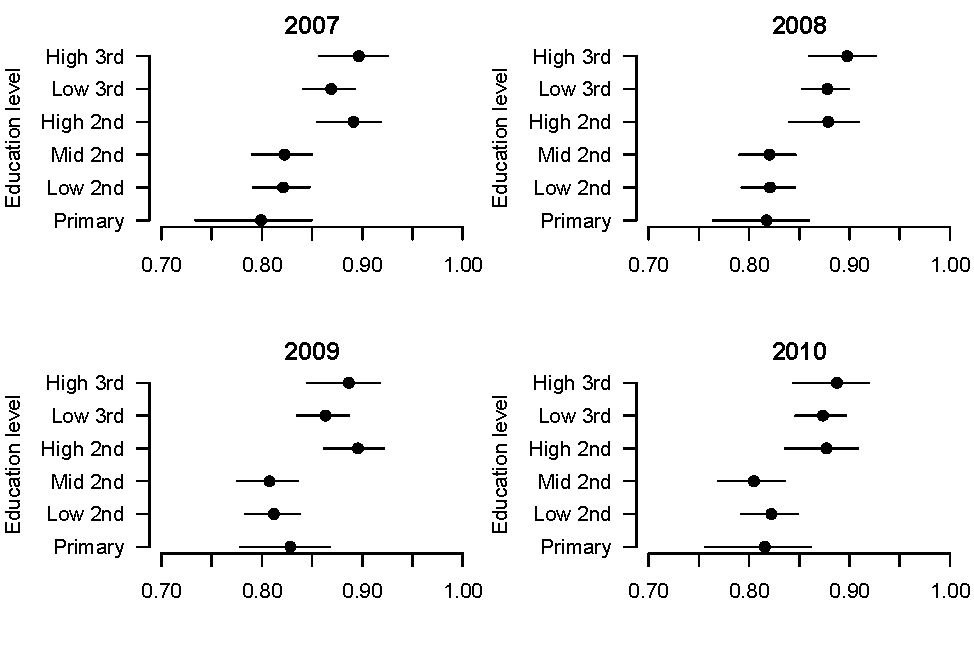
\includegraphics[width=.99\textwidth]{CI}
\label{default}
\end{center}
\end{figure}

Figure \ref{fig:ci} confirms the observations that the upper three educational groups significantly differ from the lower three groups, but
the 95\% confidence intervals within the upper and the lower three groups overlap. Due to the use of the Fisher transformation, the
confidence intervals are not symmetric around the point estimates. Another observation of interest is that none of the confidence
intervals contain 0.70, the traditional cutoff point for acceptable reliability coefficients. It can be concluded that there
are significant differences between people with higher and lower levels of education, but in all groups the reliability of self-rated health
is acceptable.

\section{Monte Carlo evaluation of the approach\label{sec:montecarlo}}

To evaluate the performance of the asymptotic standard errors and confidence intervals in the example, 
a Monte Carlo study was performed.  The multiple group model estimated in section \ref{sec:example} is taken as the true 
population model, and 512 samples from this population model were simulated\footnote{All the analyses were
performed in \R.}. Thus each sample contains six groups of different education levels, and the four observed
variables within each group are drawn from a multivariate  normal distribution with population covariance
matrix and sample size equal to the implied covariance matrix and sample size in that group from section \ref{sec:example} . 

In each of the 512 simulated samples, the model shown in figure \ref{fig:model} was estimated, and the
standardized loadings\footnote{Since the interest in this
example focuses on the standardized loadings and for the sake of brevity, we will focus only on
these standardized loadings here.} 
 (reliability coefficients) and a consistent estimate of their asymptotic variance matrix was
 calculated.
Note that the analysis is carried out separately for each of the groups, some of which have a small
sample size (see table \ref{tab:health-education}).
 We then calculated the bias in the estimates by subtracting the average standardized loading over simulations
 from the corresponding true population value given in table \ref{tab:health-education}. 
The asymptotic standard errors from table \ref{tab:health-education} were  subtracted from the 
corresponding standard deviations of the standardized estimates  over simulated samples.
 The bias in the standardized estimates and their asymptotic standard errors over the 512 simulations
 for the 24 standardized loadings is shown in table \ref{tab:montecarlo}.


\begin{table}[htb]\begin{small}
\begin{tabular}{lrrrrrrrrrrrr}
 \hline  \hline
& \multicolumn{3}{c}{2007} & \multicolumn{3}{c}{2008} & \multicolumn{3}{c}{2009} & \multicolumn{3}{c}{2010}\\
 \cline{2-13}
&	     \multicolumn{2}{c}{Bias} &  & \multicolumn{2}{c}{Bias} &  &\multicolumn{2}{c}{Bias} &  &\multicolumn{2}{c}{Bias} &  \\
\cline{2-3} \cline{5-6} \cline{8-9} \cline{11-12}
Grp&   $\hat{\tilde\l}$ & s.e & cvg. &$\hat{\tilde\l}$ & s.e & cvg. &$\hat{\tilde\l}$ & s.e & cvg. &$\hat{\tilde\l}$ & s.e & cvg. \\
  \hline
  1   &0.003 & -0.003& 95\%&0.003 & -0.002& 94\%&0.004 & -0.002& 93\%&0.003 & -0.002& 94\%\\
  2    &0.001 & 0.001& 97\%&0.001 & 0.001& 96\%&0.000 & 0.000& 96\%&0.001 & 0.000& 94\%\\
  3   &-0.001 & 0.000& 95\%&-0.001 & 0.000& 96\%&-0.001 & -0.000& 96\%&-0.000 & -0.000& 96\%\\
  4   &-0.000 & -0.000& 94\%&0.000 & -0.000& 94\%&-0.000 & 0.001& 95\%&0.000 & -0.000& 94\%\\
  5   &-0.000 & 0.000& 95\%&0.000 & -0.000& 94\%&-0.000 & -0.001& 93\%&-0.000 & -0.000& 93\%\\
  6   &0.000 & -0.001& 96\%&-0.000 & -0.000& 95\%&0.000 & -0.001& 95\%&0.001 & -0.000& 95\%\\
  \hline     \hline
\end{tabular}\end{small}
\caption{Monte Carlo results of 512 random samples taking the example model in section \ref{sec:example}  as the true model.
Shown are the bias in the standardized estimates and their asymptotic standard errors as discussed above. 
Also shown is the coverage of 95\% confidence intervals via the Fisher $z$-transformation.}\label{tab:montecarlo}
\end{table}
%  1   &0.003 & (-0.003)& 95\%&0.003 & (-0.002)& 94\%&0.004 & (-0.002)& 93\%&0.003 & (-0.002)& 94\%\\
%  2    &0.001 & (0.001)& 97\%&0.001 & (0.001)& 96\%&0.000 & (0.000)& 96\%&0.001 & (0.000)& 94\%\\
%  3   &-0.001 & (0.000)& 95\%&-0.001 & (0.000)& 96\%&-0.001 & (-0.000)& 96\%&-0.000 & (-0.000)& 96\%\\
%  4   &-0.000 & (-0.000)& 94\%&0.000 & (-0.000)& 94\%&-0.000 & (0.001)& 95\%&0.000 & (-0.000)& 94\%\\
%  5   &-0.000 & (0.000)& 95\%&0.000 & (-0.000)& 94\%&-0.000 & (-0.001)& 93\%&-0.000 & (-0.000)& 93\%\\
%  6   &0.000 & (-0.001)& 96\%&-0.000 & (-0.000)& 95\%&0.000 & (-0.001)& 95\%&0.001 & (-0.000)& 95\%\\

It can be seen in table \ref{tab:montecarlo} that the standardized loadings are unbiased estimates of the
 true population values. The absolute relative bias (not shown here) was smaller than 0.5\% in all cases.
The asymptotic standard errors are very close to the standard deviations observed over the simulations, 
although there are some deviations. 
The absolute relative bias of the standard errors as compared to the observed standard deviations 
had a maximum of 10\% (for the reliability coefficient in 2007 in the lowest educational group). 

Confidence intervals were obtained in each sample as follows: 
\begin{enumerate}
\item  The variance of $z$-transformed standardized loadings was calculated from the parameter values;
\item Standard errors of the $z$-transformed standardized loadings were used to construct a 95\%
		confidence interval for $z(\tilde\l)$;
\item The upper and lower limits of the 95\% confidence interval for $z(\tilde\l)$ were back-transformed
		to the original scale as $z^{-1}(x) = \tanh(x)$.%$z^{-1}(x) = (\exp(2x) - 1) / (\exp(2x) + 1)$.
\end{enumerate}
It was then evaluated in each sample whether the nominal 95\% confidence interval thus obtained contained the true population
value shown in table \ref{tab:health-education} or not. The percentage of samples in which this was the case is 
shown in table \ref{tab:montecarlo} in the columns marked ``cvg.''. 

Table \ref{tab:montecarlo} shows that in all cases the coverage of the 95\% confidence confidence 
intervals using the Fisher $z$-transform is close to 95\%, with the lowest observed coverage 93\%  
and the highest coverage 97\%. The mean and median coverage of the 95\% coverage intervals 
across the 24 standardized parameters are 94.7\% and 95.0\% respectively. The confidence intervals via the Fisher
$z$-transform therefore appear to perform well.

Some authors have expressed concern about the use of the normal distribution as an approximation for
the sampling distribution of standardized parameters. We therefore examined the quality of
this approximation for all standardized loadings. Figure \ref{fig:normal} presents the results for one of the 
standardized loadings in the lowest and highest educational groups.
\begin{figure}[tb]
\centering
\subfigure[Primary education]{
	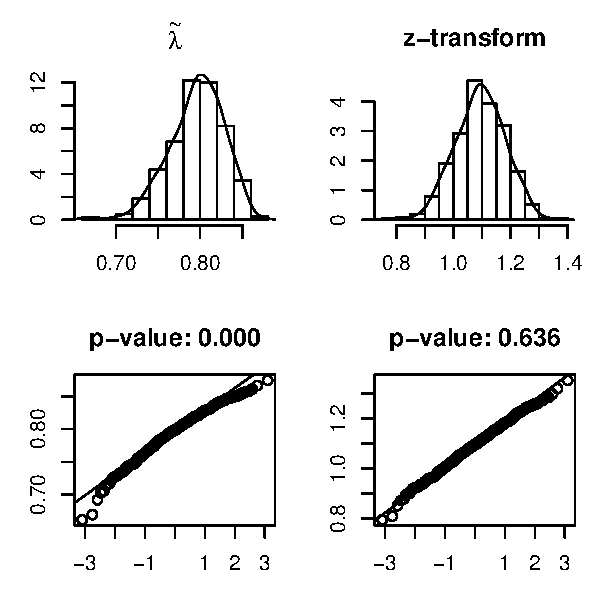
\includegraphics[width=.48\textwidth]{normplots/normality-yr1-gp1}
   \label{fig:normal-1}
 }
 \subfigure[University education]{
	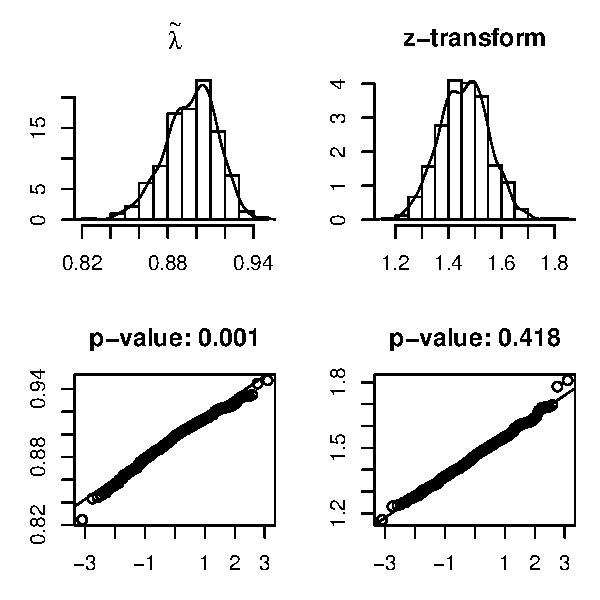
\includegraphics[width=.48\textwidth]{normplots/normality-yr1-gp6}
   \label{fig:normal-2}
 }	\caption{Distribution and normal Q-Q plots of the reliability coefficients $\tilde\l$ and their Fisher $z$-transforms
 	 in 2007 in the lowest and highest educational group.}\label{fig:normal}
\end{figure}
It can be seen in figure \ref{fig:normal} that the distribution of the raw standardized loading in both cases is somewhat skewed,
and indeed a Shapiro-Wilks test of normality is rejected in both cases. The effect appears to be more pronounced for the 
Primary group, which has the highest variance (see table \ref{tab:health-education}).
The Fisher $z$-transformed quantities do appear to follow a normal distribution in these two cases.

More generally, 9 out of 24 Shapiro-Wilks tests for the raw standardized estimates are rejected (when using
adjusted $p$-values), while none of the tests for transformed estimates are. 
Additionally, in exactly two-thirds of the cases the fit to a normal distribution is better for the transformed than for the
raw standardized values. When the normal distribution does not provide an accurate approximation 
to the sampling distribution of the standardized estimates, confidence intervals via the $z$-transformation may
still be expected to provide accurate coverage. 

This result is of course in line with the classic results for correlations
\citep[e.g.][chapter 32]{johnson1995distributions}, and indeed in the example model, the standardized loadings
are correlations: the difference in this case is that the classical theory deals with correlations between observed variables,
while the standardized loadings examined here are correlations between an observed variable and a latent variable. 
In addition, it should be clear that the presentation given here is not limited to models where the standardized parameters
represent correlations.

In summary, this short simulation study shows that for the example the suggested procedure performs well.
The standard errors for standardized parameters  are  very close to the observed standard deviation across 
the simulations. Additionally, the derived asymptotic confidence intervals via the Fisher $z$-transformation
show good coverage properties, while the sampling distribution of the  transformed standardized parameters is 
the better approximated by the normal distribution.
Note that the sample sizes in 
some of the groups are relatively small, with $n$ ranging between 256 and 799 observations (see first column of table \ref{tab:health-education}).
In spite of these smaller sample sizes the approach taken here of providing asymptotic standard errors and confidence intervals for the 
standardized estimates works well in this example.



\section{Discussion and conclusion\label{sec:conclusion}}


\marginpar{TODO: resumer intro}

In section \ref{sec:example} , we discussed an example analysis of the reliability of self-rated health in the Netherlands. Since this measure is widely used in 
 public health research, it is vital that its reliability should be acceptable. Furthermore, if correlations between self-rated health and 
 other variables are to be compared across groups with different levels of education, the reliability of self-rated health should be the 
 same across the groups. A model allowing for the estimation of reliability was therefore estimated in six groups with different levels
 of educational attainment. The reliability coefficients were obtained in the different groups, but without their standard errors the questions
 of interest could not be answered.
The example analysis of the first section therefore showed that, when standardized parameters such as reliability coefficients are of interest, it is necessary for the researcher to obtain the variance-covariance matrix of those standardized parameters in order to answer certain questions.

Although the principles applied here to obtain asymptotic standard errors and confidence intervals for standardized parameters are well-known, 
an explicit formula in terms only of the model's unstandardized parameters was not yet available. The subsequent section remedied this situation by providing this formula, deriving the Jacobian of the standardized parameters with respect to the unstandardized ones. In additional, the 
variance-covariance matrix of Fisher $z$-transformed standardized parameters was given to allow the construction of confidence intervals.

Section 4 then applied the derived equations to the unstandardized parameters obtained in the example analysis of self-rated health, shown in table \ref{tab:results-unstandardized} -- thus obtaining standard errors for the reliability coefficients (standardized loadings). Confidence intervals obtained via the Fisher $z$-transformation were also calculated. These standard errors and confidence intervals for the standardized parameters allowed for 
investigation of the hypotheses that reliability does not differ across levels of education, and that the reliability is acceptable in 
different populations (i.e. higher than 0.70). Using the derived equations, we were able to conclude that the self-rated health measure
is of acceptable reliability across groups of education, although there are significant differences in reliability between the educational groups (differential measurement error).

\marginpar{TODO: MC summary}

\vspace{12pt}
Due to the generality of SEM, the solution provided here encompasses many commonly used models as special cases. Standardized
coefficients in (multivariate) regression \citep[discussed in ][121]{bollen1990direct}, 
errors-in-variables models, factor analysis, and SUR models are special cases, for example. 
Complex sampling and non-normally distributed data can also be accommodated  \citep{muthen1995complex}. Another  application is meta-analysis of reliability coefficients as in \cite{andrews_construct_1984,scherpenzeel_validity_1997,saris_estimation_2007,alwin_margins_2007}.

Our discussion is similar to the classical work on correlations 
\citep[e.g.][chapter 32]{johnson1995distributions}; it is more general than that theory, however,
since standardized parameters in SEM may comprise not only correlations between observed variables, but
also between latent variables, multiple regression coefficients of latent and observed variables, factor loadings, 
error correlations, and $R^2$ measures.


The analytic solution to the problem of standard errors and confidence intervals for standardized parameters
 is not, of course, the only  one possible. Other approaches include
direct estimation by imposing model constraints \citep{chan2009testing}, analysis of correlation structures with constraints \citep{bentler1983covariance}, bootstrapping , likelihood-based methods, and MCMC sampling of the standardized parameters. The advantage of the method presented here is that it is uses only the unstandardized parameter estimates which result from the estimation, is  straightforward to implement in standard SEM software, and requires no further
programming from the researcher. Our Monte Carlo study suggests that the approach works well in the example given, and with
moderately small samples, but a systematic investigation of the conditions under which the approach may
be expected to perform well remains to be done.
The question of which 
method provides the most adequate approximation to the true sampling distribution of the standardized parameters therefore remains
a topic for future study.

\marginpar{TODO: final words}
In this paper we have given analytic solutions for the asymptotic variance matrices of standardized estimates in SEM and their 
$z$-transformations. These explicit solutions were not yet available in the literature. 


\begin{itemize}
\item Form of the model influences s.e. For example, adding predictors will decrease the variance of a beta: (19) and (17).
\end{itemize}

\bibliography{derivatives}
\end{document}



%%%%%%%%%%%%%%%%%%%%%%%%%%%%%%%%%%%%%%%%%%%%%%%%%%%%%%%%%
%%%%%%%%%%%%%%%%%%%%%%%%%%%%%%%%%%%%%%%%%%%%%%%%%%%%%%%%%

\appendix

\section{Calculations for the example analysis}


\begin{table}
\begin{tabular}{lrrrrrrrrrrrr}\hline\hline
	& \multicolumn{11}{c}{Unstandardized free parameters $\theta$}\\
	%\cline{2-12}
			& $\psi_{11}$ & $\psi_{22}$ &$\psi_{33}$ &$\psi_{44}$
			& $\phi_{11}$ & $\phi_{22}$ &$\phi_{33}$ &$\phi_{44}$ 
			& $\beta_{21}$ & $\beta_{32}$ &$\beta_{43}$
			\\
\hline
%\multicolumn{4}{l}{$d \vec \Lambda_s / d \vec \theta$} &\\
                   \\                                                      
$\lambda_{s, 11}$ &-0.733  & .      & .      & .     & 0.277 & .     & .     & .     & .     & .     & .   & \\
$\lambda_{s, 22}$&.     & -0.739  & .      & .     & 0.217 & 0.282 & .     & .     & 0.209 & .     & .   & \\
$\lambda_{s, 33}$&.      & .     & -0.755  & .     & 0.188 & 0.244 & 0.300 & .     & 0.180 & 0.225 & .   & \\
$\lambda_{s, 33}$&.      & .      & .     & -0.754 & 0.173 & 0.225 & 0.276 & 0.298 & 0.166 & 0.207 & 0.230\\
\\
%\multicolumn{4}{l}{$d \vec B_s / d \vec \theta$} &\\
             \\                                            
$\beta_{s, 21}$ &. & . & . & . & 0.232 & -1.059  & .      & .     & 0.223 & .     & .    & \\
$\beta_{s, 32}$&. & . & . & . & 0.131  & 0.171 & -1.147  & .     & 0.126 & 0.157 & .    & \\
$\beta_{s, 43}$&. & . & . & . & 0.058  & 0.076  & 0.093 & -1.193 & 0.056 & 0.070 & 0.077\\
\hline\hline
\end{tabular}
\caption{Derivatives of the standardized parameters $\Lambda_s$ and $B_s$ with respect
to the free parameters of the model in the quasi simplex example.}
\label{tab:jacobian}
\end{table}


\begin{table}
\begin{small}
\begin{tabular}{rrrrrrrrr}\hline\hline
	&$\psi$ & $\phi_{11}$ & $\phi_{22}$ &$\phi_{33}$ &$\phi_{44}$ & $\beta_{21}$ & $\beta_{32}$ &$\beta_{43}$  \\
\hline
  $\psi$   & \num{0.2e-4}\\
  $\phi_{11}$  & -\num{0.2e-4}  & \num{2.2e-4}\\
  $\phi_{22}$  & -\num{0.3e-4}  & \num{0.4e-4}  & \num{0.9e-4}\\
  $\phi_{33}$  & -\num{0.2e-4}  & \num{0.2e-4}  & \num{0.1e-4}  & \num{0.5e-4}\\
  $\phi_{44}$  & -\num{0.3e-4}  & \num{0.3e-4}  & \num{0.3e-4}  & \num{0.1e-4}  & \num{0.8e-4}\\
  $\beta_{21}$  & \num{0.4e-4} & -\num{1.5e-4} & -\num{0.9e-4} & -\num{0.1e-4} & -\num{0.5e-4}  & \num{4.3e-4}\\
  $\beta_{32}$  & \num{0.2e-4} & -\num{0.2e-4} & -\num{0.4e-4} & -\num{0.4e-4} & -\num{0.1e-4} & -\num{0.9e-4}   & \num{3.3e-4}\\
  $\beta_{43}$  & \num{0.3e-4} & -\num{0.3e-4} & -\num{0.3e-4} & -\num{0.3e-4} & -\num{0.7e-4}  & \num{0.4e-4}  & -\num{1.0e-4}   & \num{3.4e-4}\\
\hline\hline
\end{tabular}\end{small}
\caption{Variance-covariance matrix of the parameter estimates.}
\label{tab:vcov}
\end{table}

\vspace{12pt}

\begin{table}\begin{center}
\begin{tabular}{rrrr}\hline\hline
 Parameter & 	Estimate &	s.e. &	$z$\\
 \hline
$\lambda_{s,11}$ & 0.852& 0.006 &  134\\
$\lambda_{s,22}$ &0.851 &0.006  & 139\\
$\lambda_{s,33}$ &0.846 &0.006  & 136\\
$\lambda_{s,44}$ &0.847& 0.007  & 128\\
$\beta_{s,21}$& 0.882           &0.012 & 75\\
$\beta_{s,32}$& 0.920            &0.009 &103\\
$\beta_{s,43}$& 0.960            &0.011  &85\\
\hline\hline
\end{tabular}
\caption{Standardized parameter estimates and asymptotic standard errors for the example ($n = 3425$).}
\label{tab:vcov}\end{center}
\end{table}
\if 1=2
\begin{table}[ht]
\begin{center}
\begin{tabular}{rrrrrrrrrrrrrrr}
  \hline
 & hlt.2007 & hlt.2008 & hlt.2009 & hlt.2010 &  & hlt.2007 & hlt.2008 & hlt.2009 & hlt.2010 &  & hlt.2007 & hlt.2008 & hlt.2009 & hlt.2010 \\ 
  \hline
1 & 1.00 &  &  &  &  & 1.00 &  &  &  &  & 1.00 &  &  &  \\ 
  2 & 0.59 & 1.00 &  &  &  & 0.56 & 1.00 &  &  &  & 0.65 & 1.00 &  &  \\ 
  3 & 0.61 & 0.67 & 1.00 &  &  & 0.52 & 0.61 & 1.00 &  &  & 0.62 & 0.71 & 1.00 &  \\ 
  4 & 0.59 & 0.59 & 0.67 & 1.00 &  & 0.53 & 0.63 & 0.69 & 1.00 &  & 0.54 & 0.64 & 0.73 & 1.00 \\ 
  5 & 2.83 & 2.91 & 2.84 & 2.82 &  & 2.98 & 3.08 & 3.01 & 2.97 &  & 3.21 & 3.24 & 3.27 & 3.20 \\ 
  6 & 0.69 & 0.73 & 0.74 & 0.72 &  & 0.73 & 0.73 & 0.71 & 0.73 &  & 0.80 & 0.76 & 0.81 & 0.75 \\ 
  7 &  &  &  &  &  &  &  &  &  &  &  &  &  &  \\ 
  8 & 1.00 &  &  &  &  & 1.00 &  &  &  &  & 1.00 &  &  &  \\ 
  9 & 0.65 & 1.00 &  &  &  & 0.65 & 1.00 &  &  &  & 0.69 & 1.00 &  &  \\ 
  10 & 0.59 & 0.62 & 1.00 &  &  & 0.57 & 0.67 & 1.00 &  &  & 0.60 & 0.74 & 1.00 &  \\ 
  11 & 0.58 & 0.60 & 0.63 & 1.00 &  & 0.51 & 0.60 & 0.68 & 1.00 &  & 0.59 & 0.70 & 0.74 & 1.00 \\ 
  12 & 3.17 & 3.18 & 3.16 & 3.10 &  & 3.28 & 3.28 & 3.22 & 3.22 &  & 3.33 & 3.35 & 3.32 & 3.29 \\ 
  13 & 0.75 & 0.74 & 0.72 & 0.72 &  & 0.73 & 0.76 & 0.72 & 0.74 &  & 0.86 & 0.86 & 0.82 & 0.83 \\ 
   \hline
\end{tabular}
\end{center}
\caption{Correlations between the observed variables in each of the six groups of educational level.}
\end{table}
\fi



\section{Extension to multigroup SEM}

In multigroup SEM, let each matrix in the above equations equal the block
diagonal of the corresponding matrices in each group. 

Then define the stacking matrix $Z_{p \times pg} \definedas \left[I_p, I_p,
..., I_p\right]$. The derivatives are then 
$$
	(I_q \kronprod Z) G
$$


%
% r = P . vec(I - Psi) = 
%   = P.vec(I) - P.vec(Psi) = 
%   = P.vec(I) - P.psi 

% dr = -P dpsi

% dr/dtheta   = dr/dpsi . dpsi/dtheta
% 	    = -P.dpsi/dtheta

%var(r)	= (dr/dtheta) var(theta) (dr/dtheta)'
%	= (-P.dpsi/dtheta) var(theta) (-P.dpsi/dtheta)'
%	= P (dpsi/dtheta) var(theta) (dpsi/dtheta)' P'
%

\end{document}
